%\title{Article HW Template}

\documentclass[12pt]{article}
\usepackage{ucs}
\usepackage[utf8x]{inputenc}
\usepackage[greek,english]{babel}
\newcommand{\en}{\selectlanguage{english}}
\newcommand{\gr}{\selectlanguage{greek}}

\usepackage[paper=a4paper,top=1in, bottom=1in, right=1in, left=.7in]{geometry}

\usepackage{amsthm, amssymb, amsfonts, amsmath}
\usepackage{graphicx}
\usepackage{tikz}
\usetikzlibrary{calc,shapes}
\usepackage{enumitem}
\usepackage{mathtools}
\usepackage{mathrsfs}
\usepackage{tikz-cd}
\usepackage{hyperref, mathabx}
\usepackage{algorithm}
\usepackage{algpseudocode}
\renewcommand{\algorithmicrequire}{\textbf{Input:}}
\renewcommand{\algorithmicensure}{\textbf{Output:}}


\newcommand{\boxitem}[2]{\vspace{.55cm}
	\item[#1]
	\leavevmode
	\strut
	\vadjust{%%
		\noindent
		\raisebox{\dimexpr\dp\strutbox+\ht\strutbox+1ex}[0pt][0pt]{\tikzmark{bl}}}%%
	#2
	
	\leavevmode
	\vadjust{%
		\noindent
		\hspace*{\dimexpr\textwidth+1ex}\tikzmark{br}}%%
	
	\tikz[overlay,remember picture]{\draw[black]
		(bl) rectangle
		(br);}}

\newcommand{\tikzmark}[1]{\tikz[overlay,remember picture] \node (#1) {};}

\newcommand{\R}{\mathbb{R}}
\newcommand{\Q}{\mathbb{Q}}
\newcommand{\Z}{\mathbb{Z}}
\newcommand{\N}{\mathbb{N}}
\newcommand{\p}{\mathbb{P}}
\newcommand{\E}{\mathbb{E}}
\newtheorem*{lemma}{Lemma}
\newtheorem{llemma}{Lemma}
\newtheorem*{theorem}{Theorem}
\newtheorem*{prop}{Proposition}

\begin{document}
	\null\hfill\begin{tabular}[t]{r@{}}
		Nikolas Mavrogeneiadis - 161014\\
		gravitorious \\
		University Of West Attica \\
		Department of Informatics and Computer Engineering\\
		Professor: Panagiotis Rouvelas\\
		\today
	\end{tabular}
	\\
	\centerline{\scshape{Graph Theory-Exercise Set 3}}
	
	\begin{enumerate}[listparindent=1.5em,
		parsep = 0pt]
		
		\boxitem{1.}{
			(From Set 2 exercise 4)Let G be a simple graph. Prove that if $L(G)$ is Eulerian, then we can't conclude that G is Eulerian.
		}
		\underline{Proof:} 
		If $L(G)$ is Eulerian this means that each vertex degree of $L(G)$ is even number. This vertex will become an edge $e(v,u)$ on $G$ with $deg(v)+deg(u) = even$. In this case, we can't deduce whether $deg(v)$ and $deg(u)$ are even or not. The line graph of $K_{4}$ (on the right in the following picture) is Eulerian but the $K_4$ is not Eulerian itself (all vertices have odd degree as we can see on the left).
		This completes the proof.
		\begin{figure}[h]
			\centering
			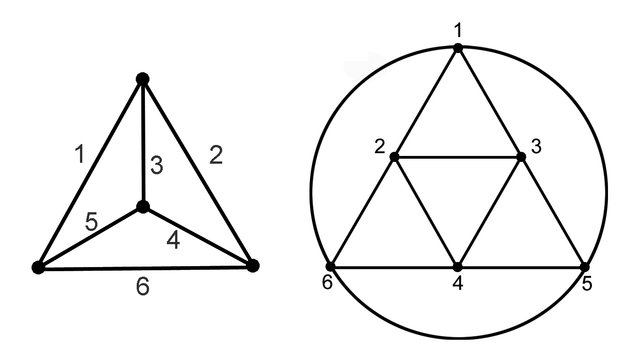
\includegraphics[width=0.55\textwidth]{ex1}
			\caption{$K_{4}$ and its Line graph}
			\label{fig:mesh1}
		\end{figure}\\
	
		\boxitem{2.}{
			\gr (Ασκηση 5 από το σετ 2)Δείξτε ότι αν ένας γράφος με τουλάχιστον 3 κορυφές που έχει απομονωμένη ή εκκρεμή κορυφή, τότε έχει μη πλήρη κλειστότητα.
		}
		Εστω μια κορυφή $v_{k}$ με $d(v_{k})\leq1$. Εστω $v_{i}$ ο προς εξέταση κόμβος για το αν θα υπάρξει ακμή $e(v_{k}, v_{i})$ στην κλειστότητα του γράφου. Προφανώς ο $v_{k}$ δεν είναι γείτονας με τον $v_{i}$ στον αρχικό γράφο. Για να υπάρξει ακμή θα πρέπει $d(v_{i}) + d(v_{k})\geq n$, δηλαδή $d(v_{i})\geq n-1$. Αυτό όμως είναι αδύνατον γιατί αν ίσχυε ότι $d(v_{i}) = n-1$ τότε οι δύο κόμβοι θα ήταν γειτονικοί στον αρχικό κόμβο, πράγμα άτοπο. Επομένως αυτοί οι δύο κόμβοι δεν θα γίνουν γειτονικοί στην κλειστότητα και άρα η κλειστότητα δεν είναι πλήρης.

		\newpage

		\boxitem{3.}{
			(Ασκηση 8 από το σετ 2) Δείξτε ότι αν ένας διμερής γράφος είναι περιττής τάξης, τότε δεν είναι Hamiltonian.
		}
		Εστω ο διμερής γράφος $K(n,m)$ για τον οποίο ισχύει ότι $n+m=odd$. Χωρίς βλάβη της γενικότητας υποθέτουμε ότι $n>m$. Θέτουμε $S_{1} = \{v_{11}, v_{12}, ..., v_{1n}\}$ το σύνολο με τις $n$ κορυφές και $S_{2} = \{v_{21}, v_{22}, ..., v_{2m}\}$ το σύνολο με τις $m$ κορυφές του $K$. Αν υπάρχει \en Hamiltonian \gr κύκλος, τότε αυτό θα πρέπει να περιέχει όλους τους κόμβους του $S_{1}$. Εστω ο $v_{1k}$ και ο $v_{1p}$ ο πρώτος και ο τελευταίος κόμβος που επισκεπτόματε από το $S_{1}$ με την προυπόθεση ότι έχουμε επισκεφθεί όλους τους κόμβους του. Το μονοπάτι αυτό είναι της μορφής $H=\{ v_{1k}, ..., v_{1p}\}$. Ομως για κάθε ζευγάρι κόμβων $(v_{1i}, v_{1(i+1)})$ του $S_{1}$ πρέπει αναγκαστικά να επισκεφθούμε έναν κόμβο του $S_{2}$. Αυτό σημαίνει ότι το $H$ περιλαμβάνει και όλους τους κόμβους του $S_{2}$ (αφού $n>m$). Για να είναι το $H$ \en Hamiltonian \gr κύκλος θα πρέπει ο $v_{1p}$ να συνδέεται με τον $v_{1k}$ κάτι το οποίο είναι αδύνατον αφού ο $v_{1p}$ συνδέεται μόνο με κόμβους του $S_{2}$ που ήδη τους έχουμε επισκεφτεί. Επομένως ο γράφος δεν είναι \en Hamiltonian.
		


		
	\end{enumerate}
\end{document}
